\chapter{Signos fermiónicos y cancelaciones supersimétricas}

\lectureoverview{La supersimetría relaciona bosones con fermiones, pero resulta más fácil entender por qué se busca una relación así antes de escribir su álgebra. Empezaremos con la topología de las rotaciones, haremos observable mediante interferencia el signo de la función de onda de un fermión, deduciremos el signo negativo de un bucle fermiónico cerrado a partir de la antisimetría bajo intercambio y, después, usaremos los signos opuestos de los bucles bosónicos y fermiónicos para motivar las cancelaciones de la energía del vacío y de la autoenergía escalar. En la segunda mitad preguntaremos cuán fuertemente puede romperse la supersimetría, cómo podrían detectarse los supercompañeros y por qué una supersimetría exacta eliminaría la estructura ordinaria de capas atómicas.}

\section{Antes de la supersimetría: una peculiaridad de las rotaciones}

La supersimetría es una simetría entre fermiones y bosones. Sin embargo, antes de intentar construirla, conviene recordar cuán distinta es la respuesta de estos dos tipos de partículas a las rotaciones. Esta cuestión parte de un hecho topológico fácil de demostrar y sorprendentemente difícil de olvidar una vez que se ha visto.

Mantén una mano con la palma hacia arriba y gira la muñeca a través de \(2\pi\). La mano recupera su orientación original, pero es evidente que el brazo no ha vuelto a una configuración equivalente: está retorcido. Continúa otros \(2\pi\), moviendo el brazo como haga falta, y podrás deshacer la torsión. Así pues, una rotación de \(2\pi\) no puede deformarse continuamente hasta quedar en ninguna rotación mientras se mantienen fijos los alrededores, mientras que una rotación de \(4\pi\) sí. La demostración con la mano es una prueba hecha con las manos en el sentido más literal.

La misma idea puede ilustrarse sin recurrir a la anatomía. Coloca una pelota dentro de una caja fija y sujétala a las paredes con cualquier número de cuerdas flexibles, elásticas, pero irrompibles. Gira la pelota una vez, un ángulo de \(2\pi\). Las cuerdas se enredan y ningún movimiento de las cuerdas por sí solas restaura la configuración original. Gira la pelota hasta completar un ángulo total de \(4\pi\) y podrás llevar las cuerdas a su alrededor hasta que desaparezca el enredo. Las paredes representan el infinito espacial: la comparación solo tiene sentido porque el contorno no gira junto con la pelota.

\begin{classroomqa}\audiencequestion{¿Se podría deshacer el enredo girando la caja? \lecturetimestamp{00:02:53}}\lecturerresponse{Eso cambiaría el problema. La caja representa el infinito espacial y se mantiene fija. Comparamos la rotación del objeto con respecto a sus alrededores, no una rotación conjunta del objeto y sus alrededores.}\end{classroomqa}

\begin{classroomqa}\audiencequestion{¿Por qué no girar simplemente la pelota otros \(2\pi\)? \lecturetimestamp{00:03:20}}\lecturerresponse{Eso es precisamente lo que distingue los dos casos. Sin volver a girar la pelota, no se puede deshacer el enredo que deja un giro de \(2\pi\). Tras el segundo giro, que completa \(4\pi\), sí se puede.}\end{classroomqa}

En el lenguaje moderno de grupos, el grupo de rotaciones tiene dos clases topológicas de caminos cerrados:
\begin{equation}
\pi_1\!\left(SO(3)\right)\cong \mathbb Z_2.
\end{equation}
Un recorrido es no trivial, pero recorrerlo dos veces da la clase trivial.
De manera equivalente, \(SU(2)\) es el recubrimiento doble de \(SO(3)\). Esta es la prehistoria geométrica del signo fermiónico.

\editorialnote{El lenguaje de \(SO(3)\), \(SU(2)\) y el grupo fundamental hace explícita la topología. Las demostraciones del brazo y de las cuerdas establecen geométricamente el mismo comportamiento de dos valores.}

\section{Qué le hace una rotación de \texorpdfstring{\(2\pi\)}{ pi2 a un estado cuántico}}

Fijemos ahora la posición de una partícula y conservemos únicamente su estado de espín, denotado por \(\ket{\psi}\). Las partículas de espín entero son bosones y las de espín semientero son fermiones. Una rotación física puede realizarse colocando un espín cargado en un campo magnético intenso y girando el campo, o haciendo que el espín precesione el ángulo deseado en un campo fijo.

\begin{classroomqa}\audiencequestion{¿Cómo se puede girar realmente el espín de un electrón en el laboratorio? \lecturetimestamp{00:05:26}}\lecturerresponse{Un campo magnético proporciona el medio para hacerlo. Se puede girar un campo suficientemente intenso para que el espín lo siga, o dejar que el espín precesione alrededor de un campo fijo. Agarrar el electrón con la mano no es un método experimental competitivo.}\end{classroomqa}

Supongamos que una rotación completa de \(2\pi\) multiplica el estado por una fase:
\begin{equation}
R(2\pi)\ket{\psi}=\xi\ket{\psi}.
\end{equation}
Al realizar la operación dos veces, se obtiene
\begin{equation}
R(4\pi)\ket{\psi}=\xi^2\ket{\psi}.
\end{equation}
Como el camino de \(4\pi\) es topológicamente trivial, en esta comparación debe actuar como la identidad. Por tanto,
\begin{equation}
\xi^2=1,
\qquad
\xi=+1\ \hbox{or}\ -1.
\end{equation}
Los bosones realizan el signo positivo y los fermiones, el negativo:
\begin{align}
R(2\pi)\ket{\psi_B}&=+\ket{\psi_B},\\
R(2\pi)\ket{\psi_F}&=-\ket{\psi_F}.
\end{align}
Para un estado de espín definido \(j\), la expresión compacta es
\begin{equation}
R(2\pi)=(-1)^{2j}.
\end{equation}
La transcripción dice brevemente que la segunda posibilidad corresponde a una multiplicación por \(2\pi\); la derivación y el argumento de la pizarra dejan claro que el factor previsto es \(-1\).

Al principio, esto parece no tener consecuencias físicas. Si cambia el signo de toda una función de onda,
\begin{equation}
\Psi\longmapsto-\Psi,
\end{equation}
las probabilidades no cambian, porque
\begin{equation}
(-\Psi)^*(-\Psi)=\Psi^*\Psi.
\end{equation}
Tomemos dos conjuntos de electrones preparados de manera idéntica. Giremos cada electrón de uno de los conjuntos un ángulo de \(2\pi\) y dejemos intacto el otro conjunto. Ninguna medición de un electrón aislado puede revelar a cuál de los dos conjuntos pertenecía. Una fase global no es observable.

\section{Hacer relativo el signo negativo}

El signo se vuelve observable cuando se impone a una rama coherente de la función de onda, pero no a la otra. Enviemos electrones de uno en uno por un aparato de dos caminos. No determinemos qué camino sigue cada electrón, pues la información sobre el camino destruye la interferencia. Sean \(\psi_1\) y \(\psi_2\) las amplitudes de los caminos superior e inferior, de modo que el estado recombinado sea
\begin{equation}
\Psi=\psi_1+\psi_2.
\end{equation}
Imaginemos por un momento que atrapamos cada rama en una región magnética. Giremos el campo asociado a la segunda rama un ángulo de \(2\pi\). Si la partícula es un fermión, el estado pasa a ser
\begin{equation}
\Psi'=\psi_1-\psi_2.
\end{equation}
Ya no se trata de un signo global. La fase relativa desplaza los máximos de interferencia y los convierte en mínimos. Si los dos paquetes que regresan son imágenes especulares respecto del centro del detector, la combinación antisimétrica se anula en el centro:
\begin{equation}
\Psi'(0)=\psi_1(0)-\psi_2(0)=0.
\end{equation}
Por tanto, el electrón nunca se detecta en ese punto de simetría. En cambio, girar ambas ramas produciría \(-\psi_1-\psi_2=-\Psi\), lo cual no tendría ningún efecto observable.

La clase destaca el carácter relacional del experimento. Girar una región magnética con respecto a la otra es análogo a girar la pelota manteniendo fija la caja. Girar ambas regiones a la vez es análogo a girar conjuntamente la pelota y la caja. Una rotación relativa de \(4\pi\) elimina el efecto porque entonces el estado fermiónico vuelve con signo positivo. Yakir Aharonov y Leonard Susskind propusieron el experimento en 1967 y, como se señala brevemente en los apuntes de clase, más tarde se realizó en forma interferométrica. El mismo principio puede aplicarse a electrones o iones cargados: un patrón de franjas desplazado identifica un estado de espín semientero, mientras que uno sin desplazar identifica un estado de espín entero.

\begin{classroomqa}\audiencequestion{Si el campo relativo se gira \(4\pi\), ¿vuelve el patrón desplazado al original? \lecturetimestamp{00:12:21}}\lecturerresponse{Sí. Dos cambios de signo se multiplican y dan \(+1\), así que desaparece la fase relativa que intercambia los máximos y los mínimos.}\end{classroomqa}

\begin{classroomqa}\audiencequestion{¿Hasta qué punto hay que tomar literalmente las cuerdas de la caja al relacionarlas con un fermión? \lecturetimestamp{00:13:43}}\lecturerresponse{Son una imagen mnemotécnica topológica, no cuerdas físicas atadas a un electrón. Un bosón se comporta como si un giro de \(2\pi\) no dejara rastro; un fermión conserva precisamente la memoria del signo representada por el enredo no trivial.}\end{classroomqa}

\begin{classroomqa}\audiencequestion{¿Hay dos electrones en las dos regiones magnéticas, uno girado y otro sin girar? \lecturetimestamp{00:14:29}}\lecturerresponse{No. Hay un único electrón en una superposición espacial coherente. Tiene una amplitud de probabilidad de ocupar cada una de las ramas, y el aparato no debe revelar cuál ocupó. Girar una región cambia una amplitud con respecto a la otra; girar ambas cambia solo la fase común.}\end{classroomqa}

El ángulo \(2\pi\) es especial porque la orientación del espín vuelve a sí misma mientras el espinor adquiere un signo. Una rotación relativa genérica también cambia la orientación del espín. Si los estados de los dos caminos regresan con estados de espín \(\ket{\chi_1}\) y \(\ket{\chi_2}\), el término de interferencia es proporcional a
\begin{equation}
\braket{\chi_1}{\chi_2}.
\end{equation}
Su módulo determina la visibilidad de las franjas.\editorialnote{}La fórmula del solapamiento de espines completa de manera estándar el análisis cualitativo de la clase sobre la pérdida parcial y total de interferencia. Los estados de espín ortogonales llevan información perfecta sobre el camino y no interfieren.

\begin{classroomqa}\audiencequestion{¿Qué ocurre si se mide en cuál de las regiones magnéticas estaba el electrón? \lecturetimestamp{00:18:03}}\lecturerresponse{El patrón de interferencia se destruye. Cualquier registro que permita distinguir los dos caminos elimina la suma coherente de sus amplitudes.}\end{classroomqa}

\begin{classroomqa}\audiencequestion{Si todos los espines parten en la misma dirección y se mide el espín final, ¿la operación de \(2\pi\) cambia esa dirección por sí misma? \lecturetimestamp{00:18:17}}\lecturerresponse{No. Después de \(2\pi\), la dirección física del espín es la misma; solo la rama fermiónica ha adquirido un signo negativo. Por eso esta operación puede cambiar la interferencia sin dejar una orientación distinta del espín que sirva como indicador del camino.}\end{classroomqa}

\begin{classroomqa}\audiencequestion{¿Qué ocurre si el campo solo se gira un ángulo de \(\pi\) en vez de \(2\pi\)? \lecturetimestamp{00:18:43}}\lecturerresponse{Entonces cambia la dirección del espín. Una rama con espín hacia arriba y otra con espín hacia abajo pueden distinguirse y no interfieren. Los ángulos intermedios reducen gradualmente la visibilidad; un giro relativo de \(180^\circ\) la destruye por completo.}\end{classroomqa}

\section{Simetría de intercambio y signo de un bucle cerrado}

La discusión de las rotaciones ha aislado un signo negativo fermiónico. Al intercambiar partículas idénticas aparece otro signo estrechamente relacionado. Para una función de onda de dos partículas,
\begin{align}
P_{12}\Psi_B(1,2)&=+\Psi_B(1,2)=+\Psi_B(2,1),\\
P_{12}\Psi_F(1,2)&=-\Psi_F(1,2)=-\Psi_F(2,1).
\end{align}
Los estados bosónicos son simétricos y los fermiónicos, antisimétricos.

\begin{figure}[htbp]\centering
\includegraphics[width=0.74\textwidth]{lecture_02_figure_02.png}\lectureframe{00:24:27}\caption{El argumento del intercambio en notación de estados. En el fotograma solo se distingue con seguridad la etiqueta del vector de estado; las ecuaciones de antisimetría aparecen escritas en el texto y no se atribuyen a la tiza que queda oculta.}\end{figure}

Ahora podemos determinar el signo relativo de un bucle cerrado de partículas sin calcular su integral. Consideremos un diagrama de Feynman del vacío, sin líneas externas. Puede imaginarse como una partícula que recorre un camino cerrado en el espacio-tiempo, o como un par partícula-antipartícula que se crea y luego se aniquila. Un diagrama de vacío de este tipo contribuye a la amplitud del vacío y, por tanto, a la energía del vacío.

Empecemos con dos copias desconectadas del bucle. Los diagramas desconectados se multiplican, así que, si un bucle tiene signo \(\sigma\), el par tiene signo
\begin{equation}
\sigma^2=+1.
\end{equation}
Cortemos ambos bucles en un instante común, por ejemplo \(t=0\). En ese instante hay dos partículas idénticas. Si las reconectamos sin intercambiarlas, reaparecen los dos bucles separados. Si intercambiamos las partículas antes de reconectarlas, la topología se convierte en un solo bucle. El intercambio aporta \(+1\) para los bosones y \(-1\) para los fermiones. Como el signo inicial de los dos bucles era positivo, los signos resultantes para un único bucle son
\begin{equation}
\begin{aligned}
\operatorname{sign}(\text{closed boson loop})&=+1,\\
\operatorname{sign}(\text{closed fermion loop})&=-1.
\end{aligned}
\end{equation}
En general, un diagrama con \(L_F\) bucles fermiónicos cerrados independientes lleva el factor
\begin{equation}
(-1)^{L_F}.
\end{equation}
La clase deduce deliberadamente esta regla a partir del intercambio, en vez de invocar la integración de Grassmann. Este argumento elemental hace visible el origen físico del signo.

\section{Signos opuestos de los bucles y energía del vacío}

Un bucle bosónico del vacío eleva la contribución del vacío con un signo, mientras que un bucle fermiónico aporta el signo opuesto. Esto resulta sugerente de inmediato, porque la densidad de energía oscura observada es extremadamente pequeña en comparación con las estimaciones ingenuas de la teoría cuántica de campos basadas en un corte. La clase cifra la discrepancia, notoria desde hace tiempo, en aproximadamente \(123\) órdenes de magnitud. El exponente preciso depende de la escala ultravioleta que se utilice; lo que perdura es la enorme discrepancia.

El valor de un bucle depende de más que la estadística. Depende de la masa, la carga, la multiplicidad y las interacciones. Sin embargo, si un bosón y un fermión coinciden en todas las propiedades pertinentes, sus contribuciones de igual magnitud pueden cancelarse:
\begin{equation}
\begin{gathered}
m_B=m_F,\qquad q_B=q_F,\qquad g_B=g_F,\\
\Delta\rho_{\mathrm{vac}}^{(B)}
+\Delta\rho_{\mathrm{vac}}^{(F)}=0.
\end{gathered}
\end{equation}
Esta observación no resuelve el problema de la constante cosmológica. Solo aporta algo que los bucles bosónicos ordinarios por sí solos no podían aportar: contribuciones de signo opuesto. En una teoría global supersimétrica exactamente no rota, las cancelaciones de la energía del vacío pueden ser exactas bajo los supuestos adecuados; una vez rota la supersimetría, el pequeño valor no nulo observado sigue sin explicación.\editorialnote{Esta precisión distingue la motivación presentada en la clase del problema, mucho más difícil, de la constante cosmológica.}

Ya sabemos que la coincidencia exacta no describe la naturaleza. Si el electrón tuviera un supercompañero de espín cero con la misma masa y carga eléctrica, la aniquilación de un electrón y un positrón a través de un fotón virtual podría producir un par de ellos:
\begin{equation}
e^-e^+\longrightarrow\gamma^*
\longrightarrow\widetilde e^-\widetilde e^+.
\end{equation}
Un escalar cargado degenerado no habría pasado inadvertido en los experimentos ordinarios de colisionadores. Así pues, la correspondencia entre bosones y fermiones no puede ser una simetría exacta del espectro observado. Se trata de una correspondencia entre tipos de partículas, no de una reflexión en el espacio físico.

\section{El objetivo más inmediato: la autoenergía escalar}

La energía del vacío es el primer ejemplo, pero la principal preocupación de la clase es la inestabilidad radiativa de las masas escalares. Un escalar que parte de masa desnuda nula puede recibir una corrección que depende cuadráticamente del corte. Esquemáticamente,
\begin{equation}
\Delta m_H^2\sim \frac{g_B^2}{16\pi^2}\Lambda^2
\end{equation}
procede de un bucle bosónico. Las masas de los fermiones cuentan con otra protección: cuando un fermión sin masa tiene una simetría quiral exacta, las correcciones radiativas no pueden generar un término de masa aditivo. Ese fue el argumento izquierda-derecha de la clase anterior.

Imaginemos ahora una simetría lo bastante rígida como para reunir un escalar y un fermión en un mismo multiplete y hacer coincidir sus interacciones. Entonces aparece un bucle fermiónico con el signo opuesto:
\begin{equation}
\Delta m_H^2
\sim
\frac{g_B^2-g_F^2}{16\pi^2}\Lambda^2+\cdots .
\end{equation}
Si la supersimetría impone \(g_B=g_F\) e igualdad de masas, los términos cuadráticos se cancelan. Así se transmite al compañero bosónico la protección de la que goza el fermión. No se trata solo de una coincidencia numérica entre dos diagramas; la simetría debe imponer la cancelación a todos los órdenes y mediante todas las interacciones permitidas.

La comparación amplia en la pizarra muestra cómo la clase pasa de bucles aislados a correcciones de bucle emparejadas para partículas que se propagan.

\begin{figure}[htbp]
\centering
\includegraphics[width=0.79\textwidth]{lecture_02_figure_04.png}
\lectureframe{00:40:23}

\medskip
\begin{tikzpicture}[scale=0.9]
\draw (-4.2,0) circle (0.55);
\draw[dashed] (-2.4,0) circle (0.55);
\draw (0,0) -- (3.7,0);
\fill (1.85,0) circle (0.055);
\draw (1.85,0) -- (1.85,0.25);
\draw[dashed] (1.85,0.85) circle (0.6);
\end{tikzpicture}\caption{Comparación general de las topologías de bucle ordinarias y las de los supercompañeros. El esquema transcrito conserva solo el contraste topológico visible; no asigna etiquetas a partículas que quedan ocultas.}\end{figure}

Tras la pausa de la clase, el argumento se retoma con lo que se llama el cuadro de orden cero. Esto no indica un orden en la teoría de perturbaciones, sino la descripción útil más esquemática:
\begin{quote}
Toda partícula tiene un supercompañero de estadística opuesta. Cada fermión tiene un compañero bosónico y cada bosón, uno fermiónico.
\end{quote}
En una teoría supersimétrica exacta, los supercompañeros también serían degenerados, es decir, tendrían la misma masa. La naturaleza no presenta esta degeneración. Aun así, si las masas son distintas pero no demasiado, la cancelación podría seguir siendo lo bastante eficaz como para evitar una corrección escalar desmesuradamente grande. Con una ruptura suave de la supersimetría, la escala peligrosa se sustituye esquemáticamente por la separación entre las masas de los supercompañeros:
\begin{equation}
\Delta m_H^2\sim
\frac{g^2}{16\pi^2}\,\Delta m_{\mathrm{SUSY}}^2
\ln\!\frac{\Lambda^2}{\Delta m_{\mathrm{SUSY}}^2}
\end{equation}
hasta factores que dependen del modelo.\editorialnote{Esta fórmula expresa la afirmación cualitativa de la clase: una correspondencia imperfecta entre masas deja una corrección residual determinada por la separación entre ellas; no es una transcripción de la pizarra.}

\section{Supersimetría rota y la apuesta experimental de 2010}

No se había observado ningún supercompañero cuando se grabó esta clase en 2010. La inferencia inmediata era que, si los supercompañeros existían, tenían que ser más pesados que las partículas conocidas y estar fuera del alcance de los aceleradores anteriores. Los modelos supersimétricos también distinguen las partículas cuyas masas solo aparecen tras la ruptura de la simetría electrodébil de los estados que pueden tener masas mayores sin romper la simetría. La clase propone esto como justificación de que la mitad visible de un espectro supersimétrico pudiera ser ligera, mientras que la mitad no observada fuera más pesada, y reconoce francamente que esta propuesta exige cierto esfuerzo de aceptación. Susskind expresa su propia expectativa de que se detectarían supercompañeros e inmediatamente aclara que es una conjetura, no un resultado.

Por tanto, el Gran Colisionador de Hadrones ocupaba un lugar central en las perspectivas que planteaba la conferencia. Se esperaba que buscara tanto el bosón de Higgs como las superpartículas. Estas afirmaciones deben leerse en su contexto de 2010: la conferencia explica la apuesta experimental antes del descubrimiento del Higgs y de los resultados posteriores de las búsquedas en el LHC.

¿Por qué un supercompañero motivado por la naturalidad no debería encontrarse a la escala de Planck? Porque en tal caso no cumpliría la función que se le asigna. Si las masas de los bosones y los fermiones difieren enormemente, las integrales de bucle dejan de cancelarse por encima de la masa menor. La corrección escalar residual queda determinada, aproximadamente, por la gran separación entre las masas y no por la escala electrodébil. La supersimetría a una escala arbitrariamente remota sigue siendo una simetría matemática, pero ya no ofrece una explicación convincente de por qué el sector de Higgs es ligero.

La clase traduce esta idea en la expectativa propia de su época de que las separaciones pertinentes entre masas debían ser del orden de unos pocos cientos de GeV y, por tanto, estar al alcance del LHC. Esta estimación numérica es histórica y depende del modelo; la cadena lógica es más importante:
\begin{equation}
\begin{gathered}
\text{Higgs protection}\\
\Downarrow\\
\text{effective boson--fermion cancellation}\\
\Downarrow\\
\Delta m_{\mathrm{SUSY}}\ \text{not too large}.
\end{gathered}
\end{equation}

\begin{classroomqa}\audiencequestion{¿Podrían cancelarse simplemente en conjunto todas las contribuciones fermiónicas con todas las contribuciones bosónicas, sin supercompañeros uno a uno? \lecturetimestamp{00:45:01}}\lecturerresponse{Podrían cancelarse numéricamente, pero sería una cancelación accidental tan finamente ajustada como el problema original. La propuesta supersimétrica es más fuerte: unos postulados razonables imponen contribuciones correspondientes, mientras que la ruptura de la supersimetría explica por qué las masas solo coinciden de manera aproximada. La energía del vacío sirvió de ejemplo; la preocupación inmediata aquí es la autoenergía del Higgs.}\end{classroomqa}

\begin{classroomqa}\audiencequestion{¿Llamar antinatural a una cancelación global presupone ya una forma reduccionista de organizar la teoría? \lecturetimestamp{00:47:51}}\lecturerresponse{Es una objeción legítima. Nadie tiene una definición definitiva de naturalidad, y la búsqueda consiste en parte en tantear en busca de una explicación convincente. La supersimetría y la ruptura espontánea de la supersimetría ofrecen marcos matemáticos conocidos que pueden imponer el patrón deseado. Queda por resolver si la naturaleza utiliza ese marco y si es único.}\end{classroomqa}

\section{Producción directa, efectos virtuales y cadenas de desintegración}

No es necesario producir una partícula pesada en su capa de masa para que influya en un experimento. Puede aparecer virtualmente dentro de un lazo y modificar ligeramente una amplitud ordinaria de dispersión electrón-positrón. Por tanto, las mediciones de precisión electrodébil imponen restricciones a las superpartículas incluso cuando la energía del centro de masas está por debajo del umbral de producción directa de pares
\begin{equation}
\sqrt{s}<2m_{\widetilde p}.
\end{equation}
La evaluación de 2010 en la conferencia es que los datos de precisión ya estaban acotando el espacio de parámetros supersimétricos, pero aún no lo habían descartado.

\begin{classroomqa}\audiencequestion{¿Se podrían inferir indirectamente los supercompañeros, como se restringieron las propiedades de partículas pesadas anteriores mediante tasas de producción precisas antes de observarlas directamente? \lecturetimestamp{00:49:01}}\lecturerresponse{Sí. Un bucle virtual de supercompañero altera ligeramente una amplitud ordinaria, así que el problema pasa a ser la fenomenología electrodébil de alta precisión, en vez de la producción directa. Sería especialmente útil un colisionador electrón-positrón limpio y con energía suficiente. Las colisiones de protones son más confusas porque el protón es un estado compuesto de quarks y gluones: en realidad colisionan sus constituyentes fluctuantes, no dos partículas elementales cuyas condiciones iniciales se conozcan con precisión.}\end{classroomqa}

Un estudiante pregunta por la reacción inversa, partiendo de abundantes superpartículas. El obstáculo no es la simetría de inversión temporal, sino la disponibilidad. Primero hay que crear los supercompañeros pesados, y se espera que la mayoría se desintegre rápidamente en estados más ligeros.

\begin{classroomqa}\audiencequestion{Si un universo contuviera muchas superpartículas, ¿podrían dos de ellas colisionar y transformarse en partículas ordinarias? \lecturetimestamp{00:53:43}}\lecturerresponse{En principio, las reacciones pertinentes tienen canales inversos, pero no se espera que los supercompañeros pesados sigan presentes en abundancia como partículas libres. Se desintegran hacia estados de menor energía, así que un experimento debe aportar primero suficiente energía de colisión para crearlos.}\end{classroomqa}

Esto plantea la cuestión de la materia oscura. En muchos modelos supersimétricos, una regla de selección discreta impide que desaparezca por completo el último supercompañero de una cadena de desintegración. En tal caso, todos los supercompañeros más pesados van desintegrándose hasta llegar al supercompañero más ligero, o LSP. Si el LSP es eléctricamente neutro, puede ser estable y difícil de detectar, lo que lo convierte en un posible candidato a materia oscura. En este intercambio, la transcripción dice una vez «energía oscura», pero la pregunta del público y la descripción de la partícula se refieren inequívocamente a la materia oscura.

\begin{classroomqa}\audiencequestion{¿Es incompatible la rápida desintegración de los supercompañeros con la propuesta de que uno de ellos podría constituir materia oscura? \lecturetimestamp{00:54:53}}\lecturerresponse{No. En los modelos que requieren un supercompañero al final de cada cadena de desintegración, la mayoría de los supercompañeros puede desintegrarse mientras el más ligero permanece estable. La carga eléctrica suele plantear dificultades fenomenológicas adicionales, así que es probable que el LSP viable sea neutro. No es indetectable en principio, pero no dejaría la señal evidente de ionización que dejaría un selectrón cargado.}\end{classroomqa}

\section{La correspondencia exige que coincidan los acoplamientos}

La correspondencia entre masas por sí sola no basta. Comparemos un bucle del vacío de un electrón con uno de un selectrón. Sus estadísticas opuestas aportan signos opuestos, pero para que las magnitudes sean iguales hace falta que las masas coincidan. Si ahora añadimos dos fotones externos, los coeficientes también contienen los acoplamientos eléctricos, así que la cancelación requiere que las cargas sean iguales:
\begin{equation}
\begin{gathered}
q_{\widetilde e}=q_e,\\
\mathcal A_{\mathrm{loop}}^{(e)}
+\mathcal A_{\mathrm{loop}}^{(\widetilde e)}=0,\\
\text{provided the full couplings match.}
\end{gathered}
\end{equation}
Una discrepancia en cualquier aspecto deja un término divergente sin cancelar. La supersimetría es valiosa porque relaciona las interacciones, además de los nombres y los espines.

\begin{figure}[H]
\centering
\includegraphics[width=0.66\textwidth]{lecture_02_figure_05.png}
\lectureframe{00:57:15}

\medskip
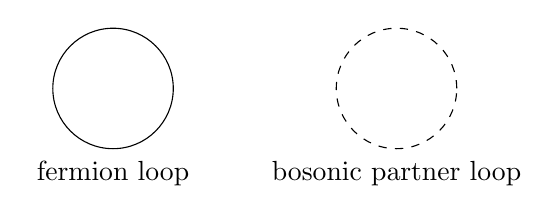
\begin{tikzpicture}[scale=0.9]
\draw (-2.0,0) circle (0.85);
\draw[dashed] (2.0,0) circle (0.85);
\node at (-2.0,-1.2) {fermion loop};
\node at (2.0,-1.2) {bosonic partner loop};
\end{tikzpicture}\caption{Comparación de bucles continuos y discontinuos durante el argumento de la correspondencia de cargas. No se reconstruyen las marcas externas recortadas, porque el fotograma por sí solo no permite determinar todos los puntos de inserción.}\end{figure}

\begin{classroomqa}\audiencequestion{¿Podrían haber pasado inadvertidos los supercompañeros sencillamente porque sus constantes de acoplamiento son distintas? \lecturetimestamp{00:56:23}}\lecturerresponse{No, si se pretende que los mismos diagramas se cancelen. Añadir interacciones con fotones permite comprobar la carga eléctrica de cada línea. Unos acoplamientos desiguales producen factores de bucle numéricos distintos y restablecen el gran residuo. La simetría debe hacer coincidir las cargas e interacciones pertinentes.}\end{classroomqa}

\begin{classroomqa}\audiencequestion{¿También debería ser sin masa el supercompañero del fotón? \lecturetimestamp{00:58:01}}\lecturerresponse{Sería sin masa en una teoría supersimétrica exacta, pues tendría la misma masa que el fotón. El mundo observado no es exactamente supersimétrico, así que un estado físico similar al fotino no tiene por qué compartir la masa del fotón.}\end{classroomqa}

\section{El diccionario de los supercompañeros}

Las reglas para formar los nombres no son elegantes, pero sí útiles. A un bosón se le asigna un compañero fermiónico cuyo nombre suele terminar en \emph{-ino}: fotón y fotino, \(W\) y wino, \(Z\) y zino, gluón y gluino, Higgs e higgsino, gravitón y gravitino. A un fermión ordinario se le asigna un compañero bosónico cuyo nombre suele empezar por \emph{s-}: electrón y selectrón, quark y squark.

\begin{center}
\begin{tabular}{@{}>{\raggedright\arraybackslash}p{0.40\linewidth}>{\raggedright\arraybackslash}p{0.52\linewidth}@{}}
\toprule
estado ordinario & supercompañero y cambio de espín\\
\midrule
Higgs escalar, \(j=0\) & higgsino, \(j=\tfrac12\); \(\Delta j=+\tfrac12\)\\
bosón gauge, \(j=1\) & gaugino, \(j=\tfrac12\); \(\Delta j=-\tfrac12\)\\
fermión de materia, \(j=\tfrac12\) & sfermión, \(j=0\); \(\Delta j=-\tfrac12\)\\
gravitón, \(j=2\) & gravitino, \(j=\tfrac32\); \(\Delta j=-\tfrac12\)\\
\bottomrule
\end{tabular}
\end{center}

La relación general es que los miembros de un supermultiplete difieren en media unidad de espín:
\begin{equation}
\Delta j=\frac12.
\end{equation}
Los ejemplos esquemáticos de la clase emparejan un fermión de materia de espín \(\tfrac12\) con un escalar, y un bosón gauge de espín uno con un gaugino de espín \(\tfrac12\). En un modelo completo con interacciones, los estados pueden mezclarse tras la ruptura de simetría, por lo que los autoestados físicos de masa quizá no conserven estos nombres más sencillos.

\begin{classroomqa}
\audiencequestion{¿Podrían todos los nuevos compañeros escalares experimentar su propia ruptura espontánea de simetría? \lecturetimestamp{01:01:27}}
\lecturerresponse{Los campos escalares pueden adquirir valores esperados, pero una ruptura de simetría adicional arbitraria tendría consecuencias fenomenológicas desastrosas. Un modelo supersimétrico viable debe organizar su potencial escalar de modo que el color, la carga eléctrica y las demás simetrías necesarias no se rompan de forma inadecuada.}
\end{classroomqa}

\begin{classroomqa}
\audiencequestion{¿Tiene el higgsino interacciones especiales correspondientes al término cuártico del Higgs? \lecturetimestamp{01:02:19}}
\lecturerresponse{La supersimetría relaciona tanto las interacciones como las partículas. La relación no se obtiene sustituyendo ingenuamente cada línea del Higgs por una línea del higgsino, pero el término cuártico escalar y las interacciones fermiónicas y auxiliares pertinentes forman parte de una misma estructura restringida. Esos detalles aún no se han desarrollado en la clase.}
\end{classroomqa}

\begin{classroomqa}
\audiencequestion{¿Hay análogos del teorema de rotación de \(2\pi\) frente a \(4\pi\) en otras dimensiones? \lecturetimestamp{01:03:07}}
\lecturerresponse{Sí, pero la dimensionalidad cambia las posibilidades. En dos dimensiones espaciales, las trayectorias de intercambio pueden enroscarse unas alrededor de otras, lo que permite la existencia de anyones cuyas fases de intercambio son más generales que las bosónicas \(+1\) y las fermiónicas \(-1\). Estas excitaciones aparecen en sistemas de materia condensada, pero quedan fuera del recorrido de este curso.}
\end{classroomqa}

\section{Por qué la supersimetría exacta borraría la química}

Por último, nos preguntamos cómo sería un mundo con supersimetría exacta. Aquí, exactitud significa que cada pareja de partícula y supercompañera tiene masas iguales e interacciones relacionadas. El electrón tendría un selectrón bosónico con la misma masa y carga eléctrica, y el fotón sin masa tendría un fotino fermiónico sin masa:
\begin{equation}
m_{\widetilde e}=m_e,
\qquad
q_{\widetilde e}=q_e,
\qquad
m_{\widetilde\gamma}=m_\gamma=0.
\end{equation}

La estructura periódica familiar de la química depende de la estadística de Fermi. El hidrógeno tiene un electrón en su orbital de menor energía. El helio acomoda allí dos porque sus etiquetas de espín son distintas. El tercer electrón del litio debe ocupar un orbital de mayor energía: el principio de exclusión de Pauli impide que tres electrones idénticos ocupen el mismo estado de una partícula. Ese electrón externo tiene más energía y tendería a caer hacia dentro, emitiendo normalmente un fotón, pero los estados inferiores, ya ocupados, bloquean la transición.

La supersimetría exacta abre otro canal:
\begin{equation}
e^-_{\mathrm{outer}}
\longrightarrow
\widetilde e^-_{\mathrm{inner}}
+
\widetilde\gamma .
\end{equation}
El electrón inicial y el fotino emitido son fermiones, mientras que el selectrón restante es un bosón. Como los selectrones obedecen la estadística de Bose y no la de Fermi, el selectrón final no queda excluido de un orbital inferior que ya esté ocupado. Por tanto, el electrón de valencia puede transformarse y caer hacia dentro.

\begin{figure}[H]
\centering
\includegraphics[width=0.62\textwidth]{lecture_02_figure_06.png}
\lectureframe{01:09:18}

\medskip
\begin{tikzpicture}[scale=0.9]
\fill (0,0) circle (0.075);
\draw (0,0) circle (0.72);
\draw (0,0) circle (1.45);
\draw[-{Latex[length=2.2mm]}] (1.42,0.2) .. controls (1.2,0.52) and (0.92,0.42) .. (0.72,0.1);
\draw[decorate,decoration={snake,amplitude=1.4pt,segment length=7pt},-{Latex[length=2.2mm]}]
  (1.58,0) -- (3.55,0);
\node[above] at (2.7,0.12) {$\widetilde\gamma$};
\node[below] at (0,-1.65) {selectron drops to a lower orbital};
\end{tikzpicture}
\caption{La transición atómica que ilustra por qué la supersimetría exacta cambiaría la química. La línea ondulada saliente es visible; su identificación como fotino procede de la transcripción.}
\end{figure}

La cuestión no se limita a un átomo parecido al litio. En un átomo grande, los electrones de valencia son los que generan la variedad química. Si pueden transformarse repetidamente en selectrones bosónicos, pueden acumularse en la región disponible de menor energía, en lugar de llenar capas. El resultado se parecería a una población bosónica concentrada cerca del núcleo, y no a la estructura familiar de los orbitales de valencia. Las moléculas formadas por enlaces direccionales y capas parcialmente llenas no conservarían una forma reconocible. La clase llama \emph{slitio} al descendiente hipotético del litio, pero la broma encierra una conclusión seria: la supersimetría exacta produciría una materia distinta de la química ordinaria y, por tanto, también de la biología ordinaria.

\begin{classroomqa}
\audiencequestion{¿Podría el acoplamiento de la transición de electrón a selectrón ser tan débil que los átomos ordinarios sobrevivieran? \lecturetimestamp{01:10:23}}
\lecturerresponse{No en la teoría exacta que estamos imaginando. La supersimetría relaciona esta transición con la interacción electromagnética, así que su acoplamiento queda fijado por la carga eléctrica y no puede elegirse libremente para que sea diminuto. La clase da una vida media aproximada del orden de un microsegundo para un átomo parecido al litio; no como cálculo de precisión, sino para subrayar que la desintegración sería rápida.}
\end{classroomqa}

Por tanto, sabemos por la materia cotidiana, al margen de las búsquedas en colisionadores, que la supersimetría no puede ser exacta a bajas energías. La separación entre las masas de las partículas y sus supercompañeras es enorme en comparación con las escalas atómica o del protón, aunque sería diminuta frente a una escala de unificación o de Planck.

\begin{classroomqa}
\audiencequestion{¿Por qué se rompe entonces la supersimetría? \lecturetimestamp{01:11:19}}
\lecturerresponse{La clase ofrece un argumento mínimo de selección: si no se rompiera, no habría observadores formados por química ordinaria que pudieran plantear la pregunta. Esto no sustituye una teoría dinámica de la ruptura de la supersimetría. Solo explica por qué un mundo de supersimetría exacta a bajas energías no podría ser el nuestro.}
\end{classroomqa}

Romper la supersimetría es matemáticamente posible y, en muchas construcciones, bastante genérico, aunque conseguir una ruptura realista dista mucho de ser automático. A la inversa, las teorías cuánticas de campos con supersimetría exacta poseen una estructura especial suficiente para que algunas puedan analizarse con mucha más profundidad que las teorías genéricas. Sirven tanto como candidatas para organizar la física de partículas como de laboratorios matemáticos excepcionalmente potentes. La próxima clase pasa de esta motivación física a explorar más a fondo esa estructura.

\section{El hilo del argumento}

El camino hacia la supersimetría ha sido deliberadamente indirecto:
\begin{enumerate}
\item Una rotación espacial de \(2\pi\) pertenece a una clase topológica no trivial, mientras que una rotación de \(4\pi\) puede deformarse hasta la identidad.
\item Un estado fermiónico adquiere un signo menos bajo \(2\pi\), y un experimento de dos caminos permite observar ese signo cuando es relativo y no global.
\item La antisimetría fermiónica bajo intercambio añade un signo menos a cada lazo fermiónico con respecto a uno bosónico.
\item Los signos opuestos de los lazos permiten cancelaciones, impuestas por la simetría, de las contribuciones al vacío y a la autoenergía escalar cuando coinciden las masas y los acoplamientos.
\item En la naturaleza no existe una correspondencia exacta. Si la supersimetría protege el sector de Higgs, su ruptura no puede hacer que los compañeros pertinentes sean arbitrariamente pesados.
\item La supersimetría exacta a bajas energías permitiría que los electrones se transformaran en selectrones bosónicos y desmoronaran la estructura de capas de la que depende la química ordinaria.
\end{enumerate}

Por tanto, la supersimetría resulta atractiva e imposible en su forma exacta más ingenua por la misma razón: vincula estrechamente los bosones y los fermiones. Esa relación estrecha puede controlar las peligrosas correcciones cuánticas, pero, si persistiera sin romperse hasta la física atómica, el mundo dejaría de parecerse al que nos rodea.